\documentclass[12pt]{article}

\usepackage[backend=biber,style=mla]{biblatex}
\usepackage[margin=1in]{geometry}
\usepackage[utf8]{inputenc}
\usepackage{setspace}
\usepackage{amsmath}
\usepackage{amssymb}
\usepackage{mathtools}
\usepackage{esint}
\usepackage{titlesec}
\usepackage{graphicx}
\usepackage{wrapfig}
\usepackage{blindtext}
\usepackage{fancyhdr}

\addbibresource{/home/krttd/Documents/UAH.bib}

%\doublespacing

\pagestyle{fancy}
\lhead{\large Skillful Python Iterables}
\chead{}
\cfoot{}
\rhead{\large\thepage}

\renewcommand*{\bibfont}{\normalsize}

\titleformat{\section}
{\Large\bf}{\thesection.\hspace{.5em}}{0em}{}%[\titlerule]

\newcommand{\bna}[2]{
        \begin{minipage}[c]{.4\textwidth}
		\begin{center}
		\includegraphics[width=\linewidth]{#1}
		\textsc{INPUT}
		\end{center}
        \end{minipage}
	\begin{minipage}[c]{.1\textwidth}
		\center\LARGE$\longrightarrow$
	\end{minipage}
        \begin{minipage}[c]{.4\textwidth}
		\begin{center}
		\includegraphics[width=\linewidth]{#2}
		\textsc{OUTPUT}
		\end{center}
        \end{minipage}\vspace{.12in}
        }

\begin{document}


\vspace*{10em}
\begin{center}
	\Huge\bf
	Skillful Python Iterables
\end{center}
\vspace{1em}
\begin{center}
	\large
	Eh 301 User Help Manual

	Mitchell T. Dodson
\end{center}

\newpage

\section{Introduction}
\label{introduction}

Python is a high-level dynamically typed object-oriented programming language rich with built-in functions as well as what its creators refer to as ``syntactic sugar,'' or small and convenient elements of the language's syntax that make solutions common programming problems easy and readable. Luxurious as these features are in implementation, to a beginner they often seem abstract and unconventional.

This manual intends to provide an introduction to several built-in functions and pieces of syntactic sugar which pertain to iterable objects such as lists, sets, and tuples. These skills enable the user to create, mutate, sort, and combine iterables clearly and easily.

The manual assumes that you have a basic understanding of object-oriented programming and the concept of functions and function references. If these concepts are unfamiliar to you, take a look at one of many free online resources such as \textsc{w3schools.com}, or check out a relevant book such as O'Reilly's \textit{Head-First Object-Oriented Analysis \& Design}

\newpage
\section{Background and Basics}
\label{background}

\subsection{what is an iterable?}
\label{what is an iterable?}

Iterables are objects in Python that form a collection of other objects. In particular, ``iterable'' referes to a type of object that allows for the notion of going to the ``next'' or ``previous'' item, in turn enabling  you to \textit{iterate} through the structure via looping and other methods.

In Python, standard iterables include (among others) lists, sets, and tuples, each of which have unique qualities. The most generalized Python iterable, \textit{lists}, are most conceptually similar to a linked list data structure. Lists are capable of containing any type and any number of objects, including repeat items, and allow you to dynamically append and remove objects at will.

Like lists, \textit{tuples} can contain any number of objects including repeat items, but items cannot be added, removed, or changed after the tuple is created (though the tuple can be converted to any other iterable type). These qualities may seem useless at first, but tuples are more memory-efficient, and allow you to more safely pass iterables to and from functions.

Finally, \textit{sets} are similar to lists in that they allow you to add, remove, or change objects at will, and to store any number of objects within, however unlike tuples and lists, sets don't allow for repeated items. As an example, if the integer \textbf{2} is already included in a set, trying to add \textbf{2} to the set will not change the set at all.

Note that the iterable type of a data structure can be changed at will by passing the structure into the identity function of the desired type. For example, to convert a tuple \texttt{my\_tuple} to a set with \texttt{set(my\_tuple)}, or a list with \texttt{list(my\_tuple)}

\subsection{python basics}
\label{python basics}

\begin{wrapfigure}{r}{.4\textwidth}
	\begin{center}
		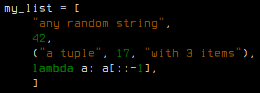
\includegraphics[width=.38\textwidth]{./figures/iterables.png}
		\caption{type-agnostic iterables}
		\label{iterables} %(to reference in the future text)
	\end{center}
\end{wrapfigure}

Unlike \textsc{C}, \textsc{C++}, or any other language that relies on dynamically-allocated memory, Python allows you to include any size and kind of object in an iterable structure with any other size and kind of object. As an example, a Python list object is happy containing 3 strings, 1 integer, even other iterables (see the tuple included in \texttt{my\_list}, Figure \ref{iterables}).

Furthermore, one of Python's core philosophies asserts that \textit{everything} is an object. This includes functions as well as static elements of data like integers or strings. The implications of this design are legion, some of which will be covered later in this manual, however for now simply bear in mind that functions can be assigned variable names or even included in iterables and other structures (see lambda, aka anonymous function included in Figure \ref{iterables}. If this is unfamiliar, don't worry; lambda functions are covered in Section \ref{lambda}).

\newpage
\section{Zip}
\label{zip}

\begin{center}
	\begin{minipage}[c]{.4\textwidth}
		\begin{center}
		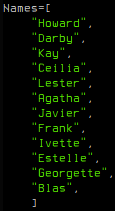
\includegraphics[height=124px]{./figures/1_zip/names.png}
		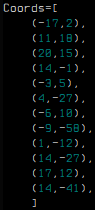
\includegraphics[height=124px]{./figures/1_zip/coords.png}
		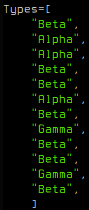
\includegraphics[height=124px]{./figures/1_zip/types.png}
		\textsc{INPUT}
		\end{center}
	\end{minipage}
	\begin{minipage}[c]{.1\textwidth}
		\begin{center}
		\LARGE$\longrightarrow$
		\end{center}
	\end{minipage}
	\begin{minipage}[c]{.4\textwidth}
		\begin{center}
		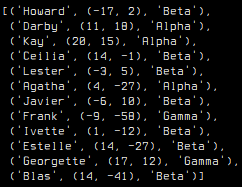
\includegraphics[height=124px]{./figures/1_zip/out_zip.png}
		\textsc{OUTPUT}
		\end{center}
	\end{minipage}\vspace{.12in}
\end{center}

\begin{wrapfigure}{r}{.6\textwidth}
	\begin{center}
		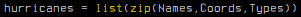
\includegraphics[width=.58\textwidth]{./figures/1_zip/codeblock_zip.png}
		\caption{zip implementation}
		\label{zip code} %(to reference in the future text)
	\end{center}
\end{wrapfigure}

When you have multiple iterables, all of which contain the same number of items, you can combine the iterables into a single iterable with items corresponding to the same indices nested in tuples therein by utilizing the \texttt{zip} built-in function.

As an example, the above input iterables, \texttt{Names}, \texttt{Coords}, and \texttt{Types} each have 12 data elements pertaining to 12 individual hurricanes such that the hurricane name at index $n$ corresponds to the coordinates at index $n$ and hurricane type at index $n$

\vspace{1em}
\noindent
\textbf{To use the `zip' function:}

\begin{enumerate}
	\item{Verify that each input iterable has the same number of items.}
	\item{Pass each iterable to the \texttt{zip()} function as a positional argument. Note that order matters here; the items of the iterable passed as first argument will be the first items to appear in the resulting tuple.}
	\item{The object returned by \texttt{zip()} is a function acts like an iterator, which cannot be parsed like a regular iterable. In order to turn it into a usable form, pass the function into an identity function as discussed in Section \ref{what is an iterable?}. In the above example, we make our new collection of nested tuples into a list.}
\end{enumerate}

\noindent
After successfully using the \texttt{zip()} built-in function, you should be left with a single new iterable of the type you chose containing tuples. Every tuple contained therein will contain one item from each input iterable corresponding to the same index as the new tuple. Furthermore, the order of appearance of items in the original iterables is conserved in the final product. If you want to change the type of the nested tuples, see \texttt{map} function (Section \ref{map}).


\newpage
\section{Map}
\label{map}

\begin{center}
\bna{./figures/2_map/in_map.png}{./figures/2_map/out_map.png}
\end{center}

\begin{wrapfigure}{r}{.4\textwidth}
	\begin{center}
		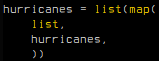
\includegraphics[width=.38\textwidth]{./figures/2_map/codeblock_map.png}
		\caption{map implementation}
		\label{map code} %(to reference in the future text)
	\end{center}
\end{wrapfigure}

Python's \texttt{map()} function gives you the opportunity to apply a function to every member of an iterable. As with many of the iterable methods covered in this manual, this is quicker, more readable, and more memory-conservative than looping manually through each member of the iterable.

Recall that \textit{everything} in Python is an object that can be passed to and called by other objects. This principle allows you to pass a function to the \texttt{map()} function \textit{as a positional argument}.

In the provided example, we use the identity function for lists as the function to apply to each item in \texttt{hurricanes}. This will convert each tuple initially nested in \texttt{hurricanes} to a nested list.

\vspace{1em}
\noindent
\textbf{To use the `map' function:}

\begin{enumerate}
	\item{Choose a function to apply individually to each item in an iterable. You may need to assign your function to a variable; otherwise, use an anonymous function (Section \ref{lambda}).}
	\item{Pass \texttt{map()} the function as the first argument, and the subject iterable as the second.}
	\item{Like the \texttt{zip()} function, \texttt{map()} returns an iterable-like object that cannot be parsed like an iterable. Simply use the identity function of the desired iterable type to turn the \texttt{map()} object into a  usable form.}
\end{enumerate}

\noindent
After successfully using the \texttt{map()} function, you will have a new iterable of the selected type with the same number of elements, such that each item will be the result of the provided function applied to item originally at that index.


\newpage
\section{Lambda}
\label{lambda}

\begin{center}
	\begin{minipage}[c]{.4\textwidth}
		\begin{center}
		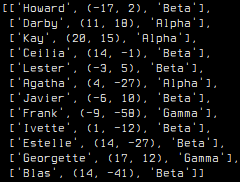
\includegraphics[height=110px]{./figures/3_lambda/in_lambda.png}
		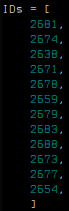
\includegraphics[height=110px]{./figures/3_lambda/ids.png}
		\textsc{INPUT}
		\end{center}
	\end{minipage}
	\begin{minipage}[c]{.1\textwidth}
		\begin{center}
		\LARGE$\longrightarrow$
		\end{center}
	\end{minipage}
	\begin{minipage}[c]{.4\textwidth}
		\begin{center}
		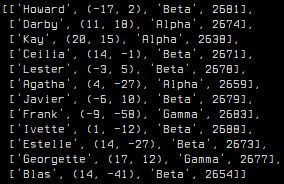
\includegraphics[height=124px]{./figures/3_lambda/out_lambda.png}
		\textsc{OUTPUT}
		\end{center}
	\end{minipage}\vspace{.12in}
\end{center}

%\begin{center}
%\bna{./figures/3_lambda/in_lambda.png}{./figures/3_lambda/out_lambda.png}
%\end{center}

\begin{wrapfigure}{r}{.4\textwidth}
	\begin{center}
		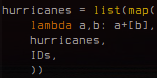
\includegraphics[width=.38\textwidth]{./figures/3_lambda/codeblock_lambda.png}
		\caption{lambda implementation}
		\label{lambda code} %(to reference in the future text)
	\end{center}
\end{wrapfigure}

Python's ``everything is an object'' design philosophy, which allows you to pass functions to other functions (as seen in Section \ref{map}) renders functions far more dynamic and accessible than in other languages. Often you will not want to create an entire function definition using \texttt{def(*args, **kwargs)} for simple functions or functions meant to be passed as arguments to other functions. Python's \texttt{lambda} method (a.k.a \textit{anonymous functions}) remedy this by enabling you to create a one-line function with any number of arguments.

Lambdas are refered to as anonymous functions because they don't require you to assign them to a variable; instead, you can define lambdas within the argument literal of whatever function you are passing them to (see Figure \ref{lambda code}).

\vspace{1em}
\noindent
\textbf{To use the `lambda' function:}

\begin{enumerate}
	\item{After the \texttt{lambda} keyword, name positional arguments separated by commas and followed by a colon (variables correspond to the order of appearance of arguments).}
	\item{After the colon, define the function's operations as you would any other function using the variables declared before the colon. These arguments are restricted to a single line.}
	\item{If you lambda is intended as be an argument to another function, simply place the lambda definition in the argument literal of the parent function. Otherwise, assign the lambda to a variable name as you would any other variable. You can pass arguments to this variable as you would a regular function.}
\end{enumerate}

\noindent
After successfully declaring a \texttt{lambda} function, you will have a function object that can be passed as an argument to other functions or assigned to any number of variables.

\newpage
\section{Sorted}
\label{sorted}

\begin{center}
\bna{./figures/4_sorted/in_sorted.png}{./figures/4_sorted/out_sorted.png}
\end{center}

\begin{wrapfigure}{r}{.4\textwidth}
	\begin{center}
		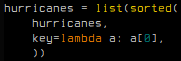
\includegraphics[width=.38\textwidth]{./figures/4_sorted/codeblock_sorted.png}
		\caption{sorted implementation}
		\label{sorted code} %(to reference in the future text)
	\end{center}
\end{wrapfigure}

Python's \texttt{sorted()} built-in function allows you to sort an iterable based on the alphabetical or numerical value of a specified key. This method is particularly useful when you have an unsorted iterable or an iterable initially sorted by a contained value other than the desired subject element.

As with \texttt{map()} and many other functions, one of the keyword arguments of \texttt{sorted()} is a function specifying which element of the iterable is the `sortable' part. In the above example, we want to sort the \texttt{hurricanes} list alphabeticlaly by the hurricane name, which is the first element of the lists nested within.

\vspace{1em}
\noindent
\textbf{To use the `sorted' function:}
\begin{enumerate}
	\item{Provide \texttt{sorted} an iterable object to be sorted as the first positional argument.}
	\item{If the first-level items in the iterable aren't the items you want to sort by, provide a function as a keyword argument with specifier ``\texttt{key=}'' that parses the item with which you want to sort the iterable.}
	\item{\texttt{Sorted} returns an iterator function object that must be converted to the desired iterable by wrapping with an identity function. In the above example, we turn the new iterable into a list using the \texttt{list()} identity function.}
\end{enumerate}

\noindent
If used properly, the \texttt{sorted()} function will return a new iterable of the specified type containing the same elements value-sorted according to the proveded key.


\newpage
\section{Filter}
\label{filter}

\begin{center}
\bna{./figures/5_filter/in_filter.png}{./figures/5_filter/out_filter.png}
\end{center}

\begin{wrapfigure}{r}{.4\textwidth}
	\begin{center}
		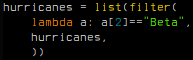
\includegraphics[width=.38\textwidth]{./figures/5_filter/codeblock_filter.png}
		\caption{filter implementation}
		\label{filter code} %(to reference in the future text)
	\end{center}
\end{wrapfigure}

Python's \texttt{filter()} built-in function allows you to reduce a provided iterable to a new iterable by applying a function to each element. If the given function evaluates `\texttt{True}' (returns anything other than \texttt{False} or \texttt{None}) when applied to an element in the original iterable, the element will be included in the new iterable returned by the function.

\texttt{filter()} functions are particularly useful when you have a large iterable containing some elements that are relevant to future operations and others which aren't. If a single operation can determine the relevance of an element (such as checking for equivalency in the example), use an anonymous function as the filter condition.

\vspace{1em}
\noindent
\textbf{To use the `filter' function:}
\begin{enumerate}
	\item{Provide either a function assigned to a variable or an anonymous function as the first positional argument. This function should evaluate `\texttt{True}' for any items you want to include in the resulting iterable.}
	\item{Provide an iterable to filter as the second positional argument. Be sure that this iterable's types are appropriate for the condition-checking function.}
	\item{\texttt{filter()} returns an iterable-like function object; in order to convert this object to something usable as an iterable, wrap the \texttt{filter} function with the identity function of the desired iterable type.}
\end{enumerate}

\noindent
If successful, this process will provide a new iterable with the same number or fewer items than the original iterable; each item will be an item that results in a `\texttt{True}' value when passed through the provided function.

\newpage
\section{Comprehension}
\label{comprehension}


\begin{center}
\bna{./figures/6_comprehension/in_comprehension.png}{./figures/6_comprehension/out_comprehension.png}
\end{center}

\begin{wrapfigure}{r}{.6\textwidth}
	\begin{center}
		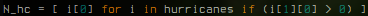
\includegraphics[width=.58\textwidth]{./figures/6_comprehension/codeblock_comprehension.png}
		\caption{comprehension implementation}
		\label{comprehension code} %(to reference in the future text)
	\end{center}
\end{wrapfigure}

Unlike the other Python built-in methods covered in this manual, Python comprehensions -- the paragon of syntactic sugar -- don't take the form of a function in the conventional sense, in that you don't pass objects and functions to a comprehension as an argument. Instead, comprehensions provide a template for defining functions and providing inputs \textit{as a single argument}. This contained function must follow a specific (but still incredibly customizable) format of statements.

\vspace{1em}
\noindent
\textbf{To use a comprehension:}
\begin{enumerate}
	\item{Wrap everything that follows in square brackets \texttt{[]} to call the comprehension method.}
	\item{Define \texttt{[ x for x in y ]} where \texttt{x} is an arbitrary variable name and \texttt{y} is the name of a predefined iterable from which the new iterable will be derived. In this case, \texttt{x} identifies the first-level elements contained within \texttt{y}.}
	\item{If you want the items included in the new iterable to be a modified version, a derived object, or a child element of the first-level items in the parent iterable, use any inline argument to specify the item that you ultimately want to include. In the above example, the first-level items from \texttt{hurricanes} are the 3-member lists assigned to \texttt{i}. Since we only want the \textit{names} of the hurricanes, we call the $0$'th index of \texttt{i}.}
	\item{If you want to filter included items based on any number of conditions, use a series of conditional statements such as \texttt{if}, \texttt{else}, \texttt{not}, et cetera. Like the \texttt{filter} bultin (Section \ref{filter}), the item will be included if and only if all the provided statements evaluate \texttt{True}.}
\end{enumerate}

\noindent
If successful, your comprehension will return a list of all the derived items that pass the given conditions. If a iterable type other than list is desired, simply convert the product using an identity function. Truthfully, this manual only scratches the surface of what comprehensions are capable of; the function is stunningly versatile, so some element of trial and error is healthy for determining the extremes of comprehensions' use cases.


\printbibliography
\end{document}
